\documentclass[conference]{IEEEtran}
\IEEEoverridecommandlockouts
% The preceding line is only needed to identify funding in the first footnote. If that is unneeded, please comment it out.
\usepackage{cite}
\usepackage{amsmath,amssymb,amsfonts}
\usepackage{algorithmic}
\usepackage{graphicx}
\usepackage{textcomp}
\usepackage{xcolor}

\def\BibTeX{{\rm B\kern-.05em{\sc i\kern-.025em b}\kern-.08em
    T\kern-.1667em\lower.7ex\hbox{E}\kern-.125emX}}
\begin{document}

\title{Concentration Effect on GaAs PIN Photodiode\\
}

\author{\IEEEauthorblockN{Mohit}
\IEEEauthorblockA{\textit{Department of Electrical Engineering} \\
\textit{Indian Institute of Technology}\\
Mumbai, India \\
20d070052@iitb.ac.in}
\and
\IEEEauthorblockN{Navneet Kumar Thakur}
\IEEEauthorblockA{\textit{Department of Electrical Engineering} \\
\textit{Indian Institute of Technology}\\
Mumbai, India \\
navneet.thakur@iitb.ac.in}
\\
\IEEEauthorblockN{ Apurba Laha}
\IEEEauthorblockA{\textit{Department of Electrical Engineering} \\
\textit{Indian Institute of Technology}\\
Mumbai, India \\
laha@ee.iitb.ac.in}
\and

\IEEEauthorblockN{Ritam Barai}
\IEEEauthorblockA{\textit{Department of Electrical Engineering} \\
\textit{Indian Institute of Technology}\\
Mumbai, India \\
20d070064@iitb.ac.in}
}
\maketitle

\begin{abstract}
In this report, the results of a simulation based on GaAs based PIN photodiode are documented and the inferences drawn from it are also reported. Parameters like the doping concentration and width of device were varied and their effects was observed on spontaneous emission and peak optical power. Relative comparison for each doping concentration was done using a plot on the same graph. \\
\end{abstract}

\begin{IEEEkeywords}
GaAs, photodiode, current, wavelength, emission, doping, junction, simulation.
\end{IEEEkeywords}

\section{Introduction}
The PIN photodiode is widely used in optical communication systems because of its high sensitivity, low noise, and quick response time. Due to its improved performance over conventional silicon (Si) based PIN photodiodes, gallium arsenide (GaAs) based PIN photodiodes have recently attracted the interest of the scientific community. In this paper, we provide an overview of GaAs-based PIN photodiodes and highlight some of their key characteristics and how they vary depending on it's parameters. The sloping shape of the conduction and valence bands, which have the maximum energy at the p-contact and the lowest at the n-contact, makes the PIN structure useful for photodiode devices.\\

The PIN photodiode is a specific type of photodetector that utilises the photoelectric effect. When light strikes the device, its semiconductor material absorbs photons to produce electron-hole pairs. Then, three distinct regions—a P-type region, an N-type region, and an intrinsic (I) region—combine to form a built-in electric field. The I area serves as a depletion region, reducing carrier diffusion and speeding up device response.\\

GaAs is a III-V compound semiconductor material that has a direct bandgap and high electron mobility. GaAs has a higher near-infrared (NIR) absorption coefficient than Si, making it suited for high-speed communication applications. GaAs-based PIN photodiodes are more responsive and noise-free than Si-based equivalents because of their lower size and increased carrier mobility.\\

In this report, we are mainly focussing on modelling a GaAs based PIN photodiode, using the COMSOL software.

\begin{figure}
\begin{center}
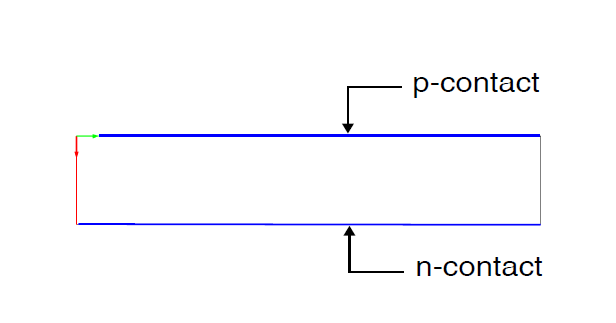
\includegraphics[scale = 0.4]{Structure.png}
\caption{The device geometry is a simple rectangle with a p-contact on the top surface and an n-contact on the bottom surface.Source: COMSOL documentation for GaAs PIN photodiode simulation}
\end{center}
\end{figure}

\begin{figure}
\begin{center}
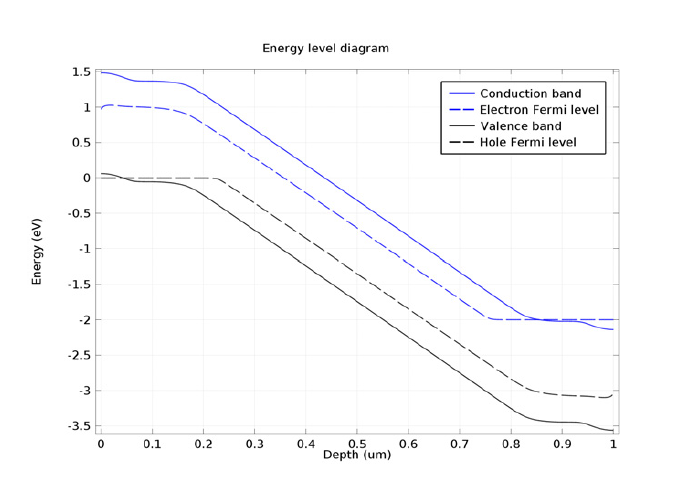
\includegraphics[scale = 0.4]{Energy.png}
\caption{The resulting energy level diagram, taken along the red arrow indicated in the geometry diagram, showing the band edges and the quasi-Fermi levels. In the intrinsic region the quasi-Fermi electron level is below the conduction band and the quasi-Fermi hole level is above the valence band. This means that the conduction band is empty whilst the valence band is full, making this region well suited to absorbing photons. Source: COMSOL documentation for GaAs PIN photodiode simulation}
\end{center}
\end{figure}



\section{Model and Method Followed}
In this model, we are making a simple rectangular GaAs PIN photodiode i.e a we are modelling a 3D model into a 2D model using the COMSOL software. Firstly we are taking a COMSOL documentation on GaAs PIN photodiode and building upon it by varying tha parameters and then we are comparing that with the original observations. To understand the PIN better we will first see the principle of PIN model. An electron and a hole are produced when a photon is absorbed in a GaAs-based PIN photodiode. The hole is then swept in the opposite direction, towards the p-contact, while the electron is swept in the direction of the n-contact. The n-contact is set to 2 V and the p-contact is grounded, indicating reverse bias mode for the device. Due to the fact that a current is produced by using the absorbed light, this mode of operation is frequently referred to as the photoconductive mode. The current produced for a given incident light wavelength is linearly proportional to the irradiance. The width of the depletion layer and the slope of the energy levels both increase due to the reverse bias, which also shortens the reaction time. However, this has the drawback of increasing the dark current, as the bias causes more current to flow when there is no light.[1]\\

We use semiconductor interface for the doping and electrical contacts whereas Electromagnetic Waves, Frequency Domain (EWFD) for the incident electromagnetic radiation and to couple these two interfaces optical transitions are used. In this model we are computing the absorption rate using a direct band gap model with an approximation that it has parabolic bands. A major result that we observe in this is the spontaneous emission which is calculated using the lifetime of electron-hole pairs within the material. We can also calculate the interaction strength between states in the conduction and valence bands.The visualisation gains a new dimension in the frequency domain, allowing for the display of some attributes as functions of photon energy. The spontaneous emission spectra are frequently plotted using this method. A generation term for electrons and holes is added to the carrier continuity equations when photons are absorbed in a semiconductor, changing the material's susceptibility. The Semiconductor-Electromagnetic Waves Coupling feature, found under the Multiphysics node in the model builder tree, automatically couples the p-contact and n-contact interfaces in the simulation model. This function configures the absorption in the semiconductor interface to use the electric field from the Electromagnetic Waves, Frequency Domain interface as the input. In order to account for the adjustments calculated in the Semiconductor interface, it also modifies the susceptibility in the Electromagnetic Waves, Frequency Domain interface.[1]\\

For this model, we have prepared different devices for each doping concentration, and then a wavelength vs power plot is observed. The observations observed and how the observations were made are given in the following section.


\begin{figure}
\begin{center}
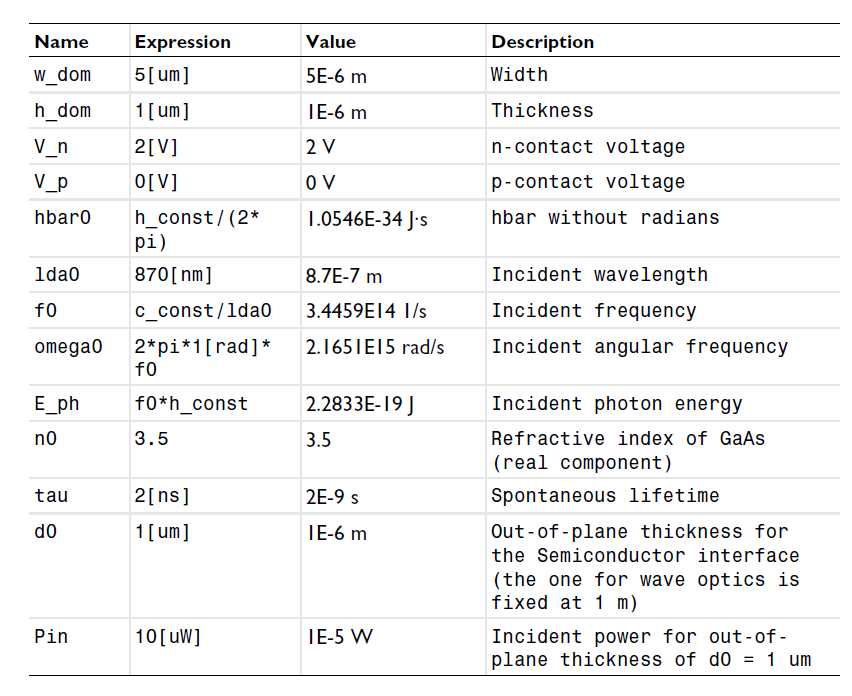
\includegraphics[scale = 0.4]{Param.png}
\caption{Model original parameters. Source: COMSOL documentation for GaAs PIN photodiode simulation}
\end{center}
\end{figure}


\section{Results and Observations}
Now we will look into the results that we got from the simulation.

\subsection{Current vs Wavelength}

\begin{figure}
\begin{center}
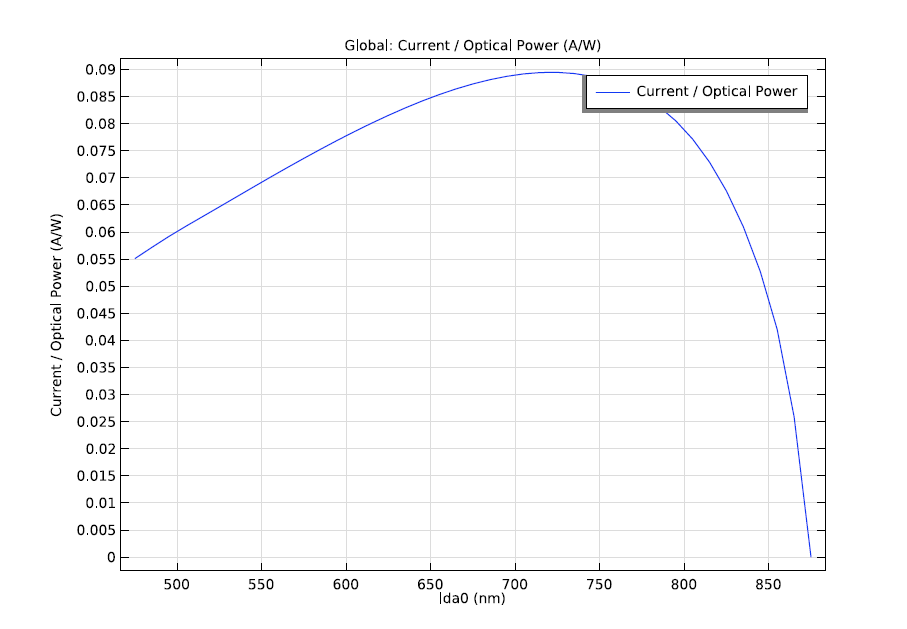
\includegraphics[scale = 0.3]{Current.png}
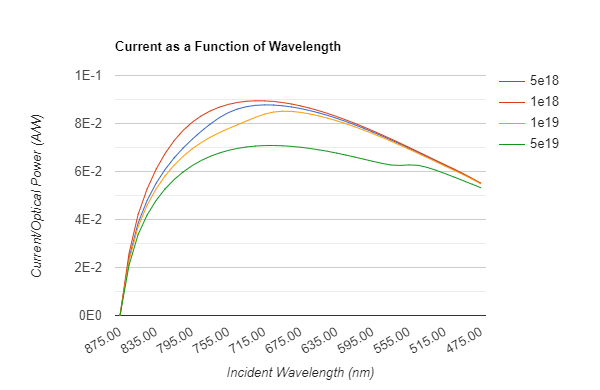
\includegraphics[scale = 0.4]{Current as f(W).png}
\caption{Top - Current output per input optical power as a function of the incident wavelength. Source: COMSOL documentation for GaAs PIN photodiode simulation. Bottom - The experimental result that was observed for each doping concentration}
\end{center}
\end{figure}


The resultant plot can be seen in the figure [4] in which we have plotted the current through the device per unit input optical power as a function of the incident photon wavelength. The inferences that can be drawn from the plot is that, when the wavelength is large there is not much current which is also correct because wavelength is inversely proportional to energy so higher wavelength means lower energy so if this energy is below the bandgap then it is expected that it will not get absorbed. Now as we decrease the wavelength, the energy increases so the current increases very fast, at a particular wavelength but after that it again starts reducing for lower wavelength because incident power is constant so with increasing photon energy the rate of photons decreases. The current depends on the product of absorption probability and rate of incident photons.\\

Current $\propto$ Probability x Rate of incident photons \\

Now if we compare the currents for different doping concentrations then we observe that as we increase the current the maximum current decreases. This is due to a phenomenon known as carrier depletion, which occurs when the doping concentration is high enough to remove most of the free charge carriers (electrons and holes) from the region.\\
Also we see that in general the wavelength at which current peak is observed is reducing. This is because the bandgap of the semiconductor is dependent on the doping concentration, and the bandgap determines the energy of the photons that can be absorbed by the device.

\subsection{Spontaneous Emission}

\begin{figure}
\begin{center}
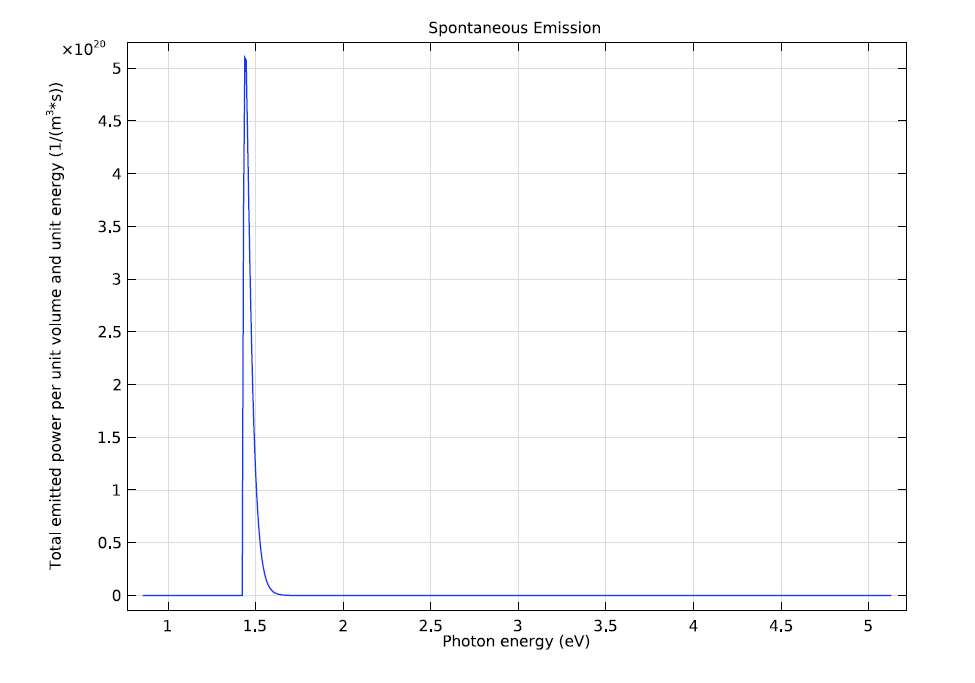
\includegraphics[scale = 0.3]{Spont.png}
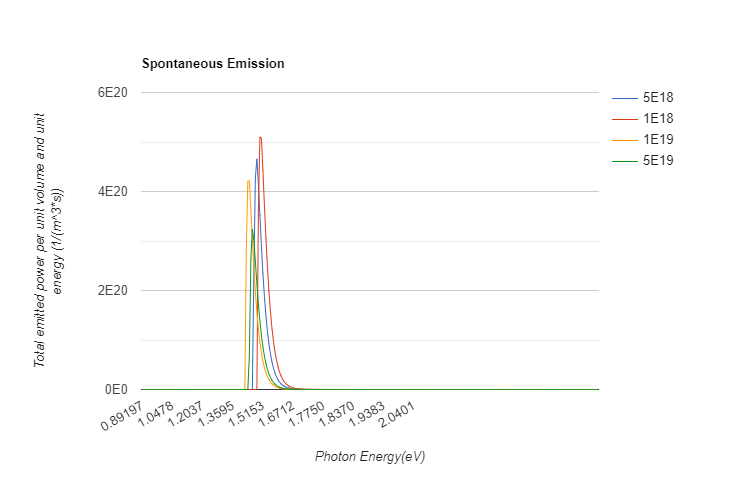
\includegraphics[scale = 0.4]{spont emission.png}
\caption{Top - Spontaneous emission from the device when the incident wavelength is set to 725 nm. Source: COMSOL documentation for GaAs PIN photodiode simulation. Bottom - The experimental result that was observed for each doping concentration}
\end{center}
\end{figure}

The resultant plot can be seen in the figure [5] in which we have plotted the spontaneous emission from the device for the incident wavelength being the one for which we got the maximum current. Now from the plot some general things observed are that there are no emissions below the band-gap energy which is what we expect. At the band-gap energy the emission starts abruptly and after that it again dies off this is because both above and below the band gap the number of available electronic states again becomes limited due to which there is less emission.\\

Now if we compare the spontaneous emissions for different doping concentrations then we observe that total emitted power decreases as we increase the concentration this is because increasing the doping concentration of a GaAs PIN photodiode leads to an increase in the density of impurities and defects in the crystal lattice, which can act as recombination centers and reduce the carrier lifetime. Therefore, the likelihood of an electron-hole pair recombining through spontaneous emission reduces with a shorter carrier lifetime as a result, when the doping concentration increases, the power released through spontaneous emission decreases.


\subsection{Doping Profile}


\begin{figure}
\begin{center}
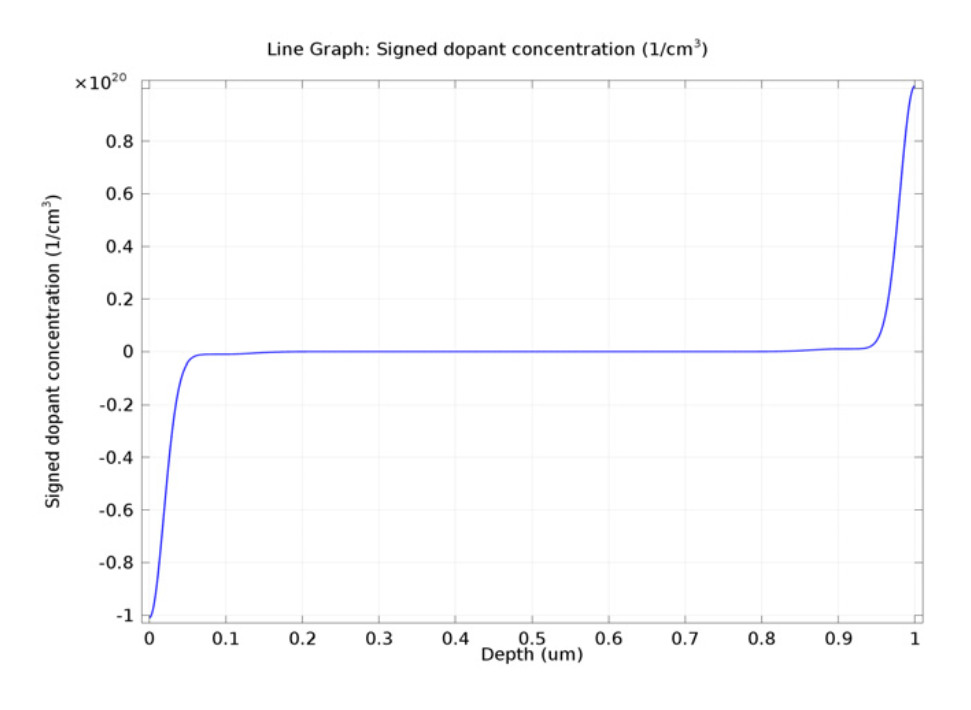
\includegraphics[scale = 0.3]{Dopant.png}
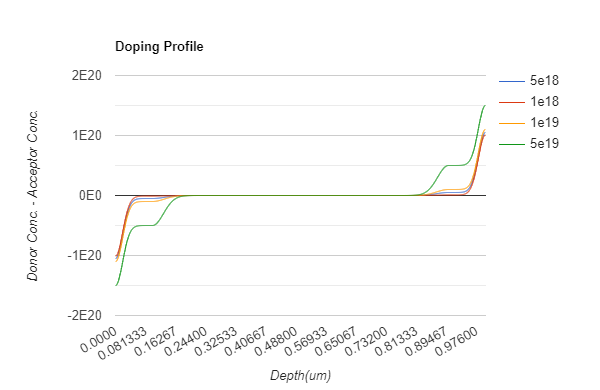
\includegraphics[scale = 0.4]{doping profile.png}
\caption{Top - Signed dopant concentration where Negative values correspond to net p-type doping and positive values correspond to net n-type doping. The PIN dopant profile is clearly visible, with highly doped p and n-type layers adjacent to the top and bottom surface, respectively. There is a wide intrinsic (undoped) region between approximately 0.15 and 0.85 um from the surface. Source: COMSOL documentation for GaAs PIN photodiode simulation. Bottom - The experimental result that was observed for each doping concentration}
\end{center}
\end{figure}



The resultant plot can be seen in the figure [6] in which we have plotted the dopant profile vs the depth from n contact to p contact. In the plot negative values correspond to p-type and vice versa. Also there is a wide range of undoped region between the top and bottom surface.\\

Now if we compare the dopant profile for different doping concentrations then we observe that as we increase the doping concentration the dopant concentration increases on both sides i.e. top and bottom. This is because the fermi level rises above the conduction band so the doping profile remains constant for a bit in between and then it again rises similarly for valence band but vice versa.

\subsection{Energy Level Diagram}

The resultant plot can be seen in the figure [7] in which we have plotted the Energy level diagram of the device for different doping concentrations displaying the quasi-Fermi levels and band boundaries. The quasi-Fermi electron level and quasi-Fermi hole level are above and below the conduction band and valence band, respectively, in the intrinsic region. As a result, the valence band is full and the conduction band is vacant, making this region ideal for absorbing photons.\\

\begin{figure}
\begin{center}
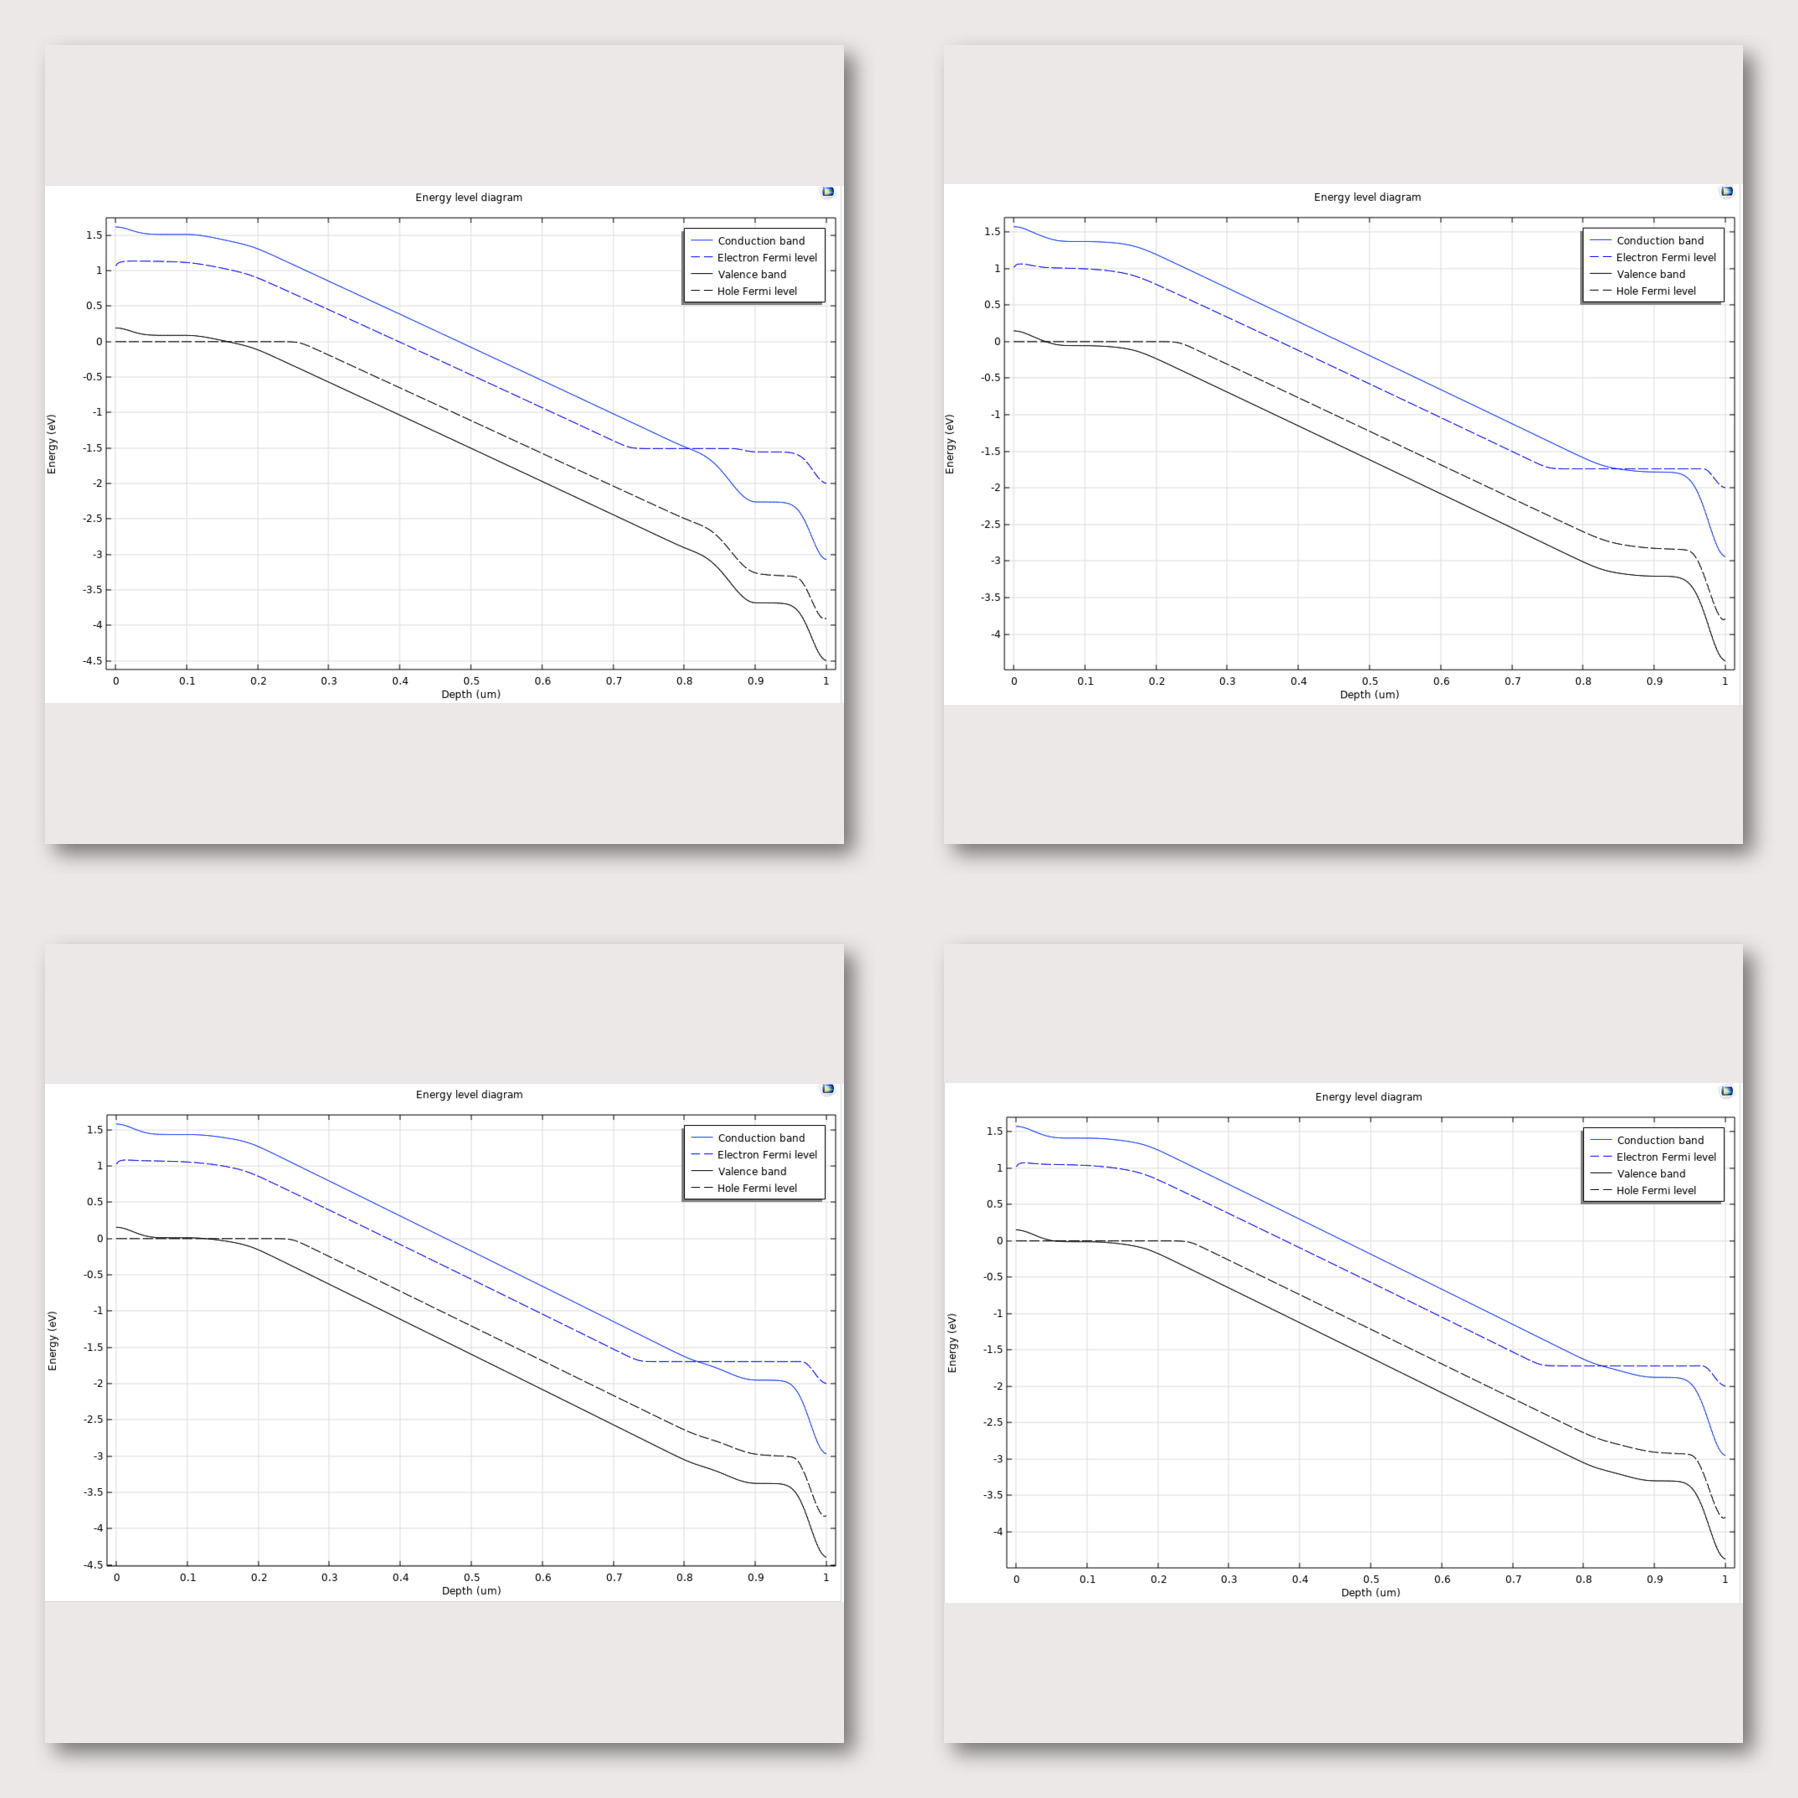
\includegraphics[scale = 0.15]{Fermi.jpeg}
\caption{Top Left - 5e19. Top Right - 1e18. Bottom Left - 1e19. Bottom Right - 5e18.}
\end{center}
\end{figure}

From the plot we can observe that as we increase the concentration, the electron fermi level rises above the conduction band for higher depth whereas the valence band rises above the hole fermi level for lower depth. This is because as electron and hole concentration increases, the density of states in the valence and conduction bands, respectively, determines how electrons and holes are distributed.\\

Higher i-region depths cause the electron Fermi level to climb above the conduction band because the density of states in the conduction band is higher than the electron concentration. This shows that the semiconductor is n-type and the surplus electrons are the dominant carriers at these depths. In contrast, the valence band rises above the hole Fermi level at lower depths where the density of states is lower than the hole concentration.

\subsection{Observed Parameters}

Given in figure [8] are the expressions that are used to calculate the parameters: absorption rate and charged particle arrival time. The results obtained from these calculations can be seen in Table 1 and we can observe that there is a conservation of particles in which the number of particles absorbed on port (contact) is nearly same as the number of particles absorbed due to optical transition.

\begin{figure}
\begin{center}
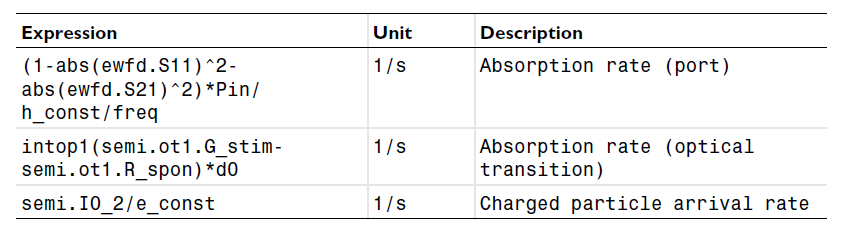
\includegraphics[scale = 0.4]{Calc.png}
\caption{The expressions for Absorption rate of port, arrival time and charged particle arrival time. Source: COMSOL documentation for GaAs PIN photodiode simulation.}
\end{center}
\end{figure}
\begin{table}[htbp]
\caption{Observed Model Parameters}
\begin{center}
\begin{tabular}{|c|c|c|c|c|}
\hline
\textbf{Doping} & \textbf{lda0 (m)}& \textbf{ Absorption}& \textbf{Absorption }& \textbf{Charged} \\
\textbf{Conc-} & & \textbf{Rate}& \textbf{Rate}& \textbf{particle} \\
\textbf{entra-} & & \textbf{(Port)}& \textbf{(Optical}& \textbf{arriving} \\
\textbf{tion} & & \textbf{(1/s)}& \textbf{(Transition}& \textbf{rate (1/s)} \\
\hline
1e18& 7.25E-7 & 5.586788E12 & 5.586735E12  & 5.584E12  \\
\hline
5e18& 7.150E-7 & 5.483145E12  & 5.483009E12 & 5.477E12 \\
\hline
1e19& 6.9500E-7 &  5.320554E12 & 5.320400E12 & 5.312E12  \\
\hline
5e19& 7.05E-7 &  4.424895E12 & 4.424866E12 & 4.421E12  \\
\hline

\end{tabular}
\label{tab1}
\end{center}
\end{table}




\section{Conclusion}
In summary, the goal of this simulation experiment was to examine the functionality of a GaAs-based PIN photodiode. We examined the device's output power and  performance using the simulation, and we were able to optimise the device's characteristics for optimum performance.\\

This simulation experiment offers useful information about the creation and improvement of GaAs-based PIN photodiodes for a range of applications. The results of the simulation might be experimentally verified in the future study, and the device's settings could be further optimised for certain uses.

\section*{Acknowledgment}

We would like to thank our mentor's Professor Apurba Laha and research assistant Navneet Kumar Thakur for their continuous support and guidance throughout this project.


\begin{thebibliography}{00}
\bibitem{b1} COMSOL Documentation for GaAs PIN Photodiode
\bibitem{b2} @article{article,
author = {Yosif, Bedir and Abo-Elsoud, Mohy and Marouf, Hagar},
year = {2020},
month = {10},
pages = {},
title = {High-Performance Enhancement of a GaAs Photodetector Using a Plasmonic Grating},
journal = {Plasmonics},
doi = {10.1007/s11468-020-01142-6}
}

\end{thebibliography}


\end{document}
